\section{GMM vs Supervectors}

[GMM vs supervectors] Adapt K-Means

\begin{figure}[H]
	\centering
	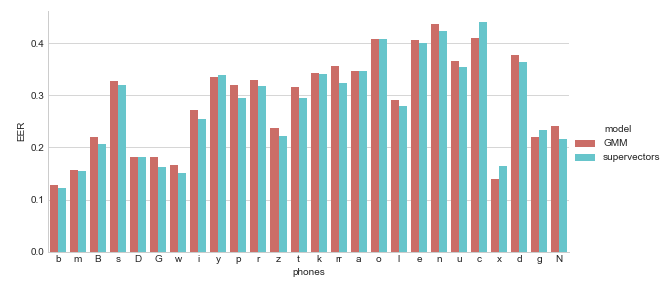
\includegraphics[width=0.6\textwidth]{files/figures/results/gmm-vs-supervectors/gmm-vs-supervectors-dev.png}
\end{figure}

\begin{figure}[H]
	\centering
	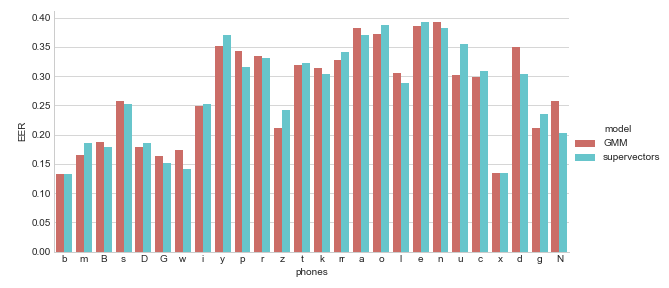
\includegraphics[width=0.6\textwidth]{files/figures/results/gmm-vs-supervectors/gmm-vs-supervectors-heldout.png}
\end{figure}


\section{Legendre Best System}

\begin{figure}[H]
	\centering
	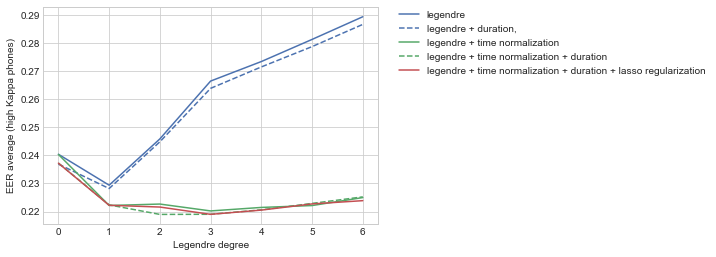
\includegraphics[width=0.8\textwidth]{files/figures/results/legendre-dct/legendre-tunning.png}
\end{figure}


\section{Legendre vs DCT}

\begin{figure}[H]
	\centering
	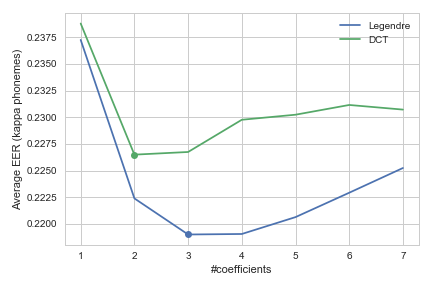
\includegraphics[width=0.5\textwidth]{files/figures/results/legendre-dct/legendre-dct-coefficients.png}
\end{figure}


\section{Fusion systems}

\subsection{Statistical Significant Filtering}

\subsection{Plots}

\begin{figure}[H]
	\centering
	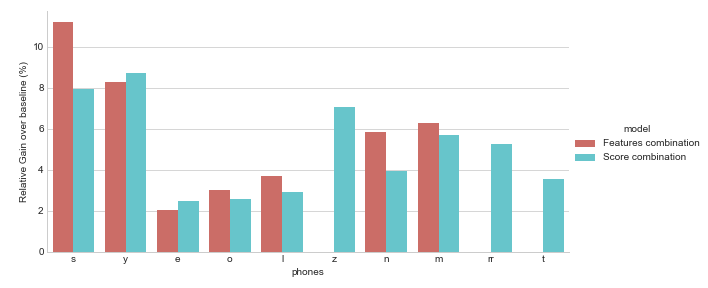
\includegraphics[width=0.6\textwidth]{files/figures/results/relatives/relatives-fusion-systems-dev-mcnemar.png}
\end{figure}

\begin{figure}[H]
	\centering
	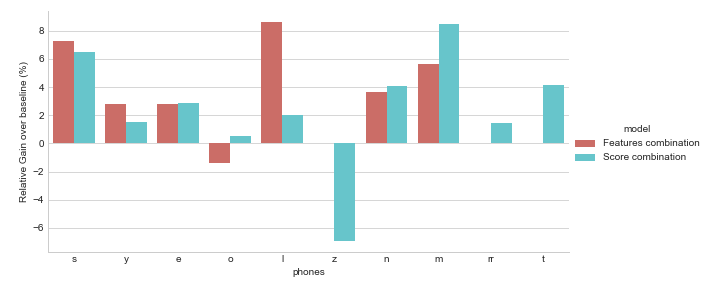
\includegraphics[width=0.6\textwidth]{files/figures/results/relatives/relative-fusion-systems-heldout-mcnemar.png}
\end{figure}
